\documentclass[dvipsnames]{article}
\usepackage[english]{babel}
\usepackage{multirow}
\usepackage[letterpaper,top=2cm,bottom=2cm,left=3cm,right=3cm,marginparwidth=1.75cm]{geometry}
\usepackage{amsmath}
\usepackage{graphicx}
\usepackage{minted}
\usepackage{amsthm}
\usepackage{mathtools}
\usepackage[colorlinks=true, allcolors=blue]{hyperref}
\usepackage{fancyhdr}
\usepackage{enumerate}
\usepackage{tikz-cd}
\usepackage{mdframed}

\newmintinline[java]{java}{}

\usepackage{tikz}
\usetikzlibrary{shapes}
\usetikzlibrary{arrows}

\tikzset{
  treenode/.style = {align=center, inner sep=0pt, text centered,
    font=\sffamily},
  avl_node/.style = {treenode, circle, black, draw=black,
    text width=1.5em, very thick},% arbre rouge noir, noeud rouge
  black_node/.style = {treenode, circle, white, font=\sffamily\bfseries, draw=black,
    fill=black, text width=1.5em},% arbre rouge noir, noeud noir
  red_node/.style = {treenode, circle, red, draw=red,
    text width=1.5em, very thick},% arbre rouge noir, noeud rouge
  nil_leaf/.style = {treenode, rectangle, draw=black, fill=black,
    minimum width=0.3em, minimum height=0.3em}% arbre rouge noir, nil
}

\begin{document}
\section*{Week 10. Problem set (solutions by \textcolor{blue}{Karim Khabibrakhmanov})}

\thispagestyle{fancy}
\lhead{Karim Khabibrakhmanov (\texttt{k.khabibrakhmanov@innopolis.university}), group B24-DSAI-05}

\begin{enumerate}

  \item Consider the following directed graph $\mathcal{G}_1$ and answer questions:
  
  \begin{center}
  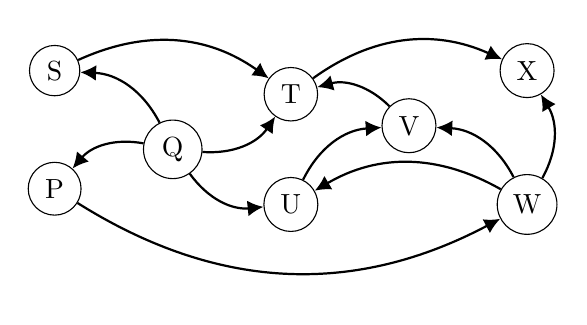
\begin{tikzpicture}
  
  \tikzset{vertex/.style = {shape=circle,draw,minimum size=1.5em}}
  \tikzset{edge/.style = {-{Latex[length=2mm,width=2mm]},thick}}
  % vertices
  \node[vertex] (a) at  (0,0.5) {P};
  \node[vertex] (b) at  (1.5,1) {Q};
  \node[vertex] (c) at  (0,2)   {S};
  \node[vertex] (d) at  (3,1.7) {T};
  \node[vertex] (e) at  (3,0.3) {U};
  \node[vertex] (f) at  (4.5,1.3) {V};
  \node[vertex] (g) at  (6,0.3)   {W};
  \node[vertex] (h) at  (6,2)   {X};
  %edges
  \draw[edge] (b) to[bend right] (a);
  \draw[edge] (b) to[bend right] (c);
  \draw[edge] (b) to[bend right] (d);
  \draw[edge] (c) to[bend left] (d);
  \draw[edge] (d) to[bend left] (h);
  \draw[edge] (b) to[bend right] (e);
  \draw[edge] (f) to[bend right] (d);
  \draw[edge] (e) to[bend left] (f);
  \draw[edge] (g) to[bend right] (e);
  \draw[edge] (g) to[bend right] (f);
  \draw[edge] (g) to[bend right] (h);
  \draw[edge] (a) to[bend right] (g);
  \end{tikzpicture}
  \end{center}

  \begin{enumerate}
    \item Write down \textbf{all} possible topological sortings for the vertices of $\mathcal{G}_1$.

    \color{blue}
    \textbf{Answer:}\\
    \textbf{1.}
        \begin{tabular}{|c|c|c|c|c|c|c|c|}
            \hline
              \makebox[\widthof{0}][c]{Q}
            & \makebox[\widthof{0}][c]{S}
            & \makebox[\widthof{0}][c]{P}
            & \makebox[\widthof{0}][c]{W}
            & \makebox[\widthof{0}][c]{U}
            & \makebox[\widthof{0}][c]{V}
            & \makebox[\widthof{0}][c]{T}
            & \makebox[\widthof{0}][c]{X}
            \\
            \hline
        \end{tabular}\\
    \textbf{2.}
        \begin{tabular}{|c|c|c|c|c|c|c|c|}
            \hline
              \makebox[\widthof{0}][c]{Q}
            & \makebox[\widthof{0}][c]{P}
            & \makebox[\widthof{0}][c]{S}
            & \makebox[\widthof{0}][c]{W}
            & \makebox[\widthof{0}][c]{U}
            & \makebox[\widthof{0}][c]{V}
            & \makebox[\widthof{0}][c]{T}
            & \makebox[\widthof{0}][c]{X}
            \\
            \hline
        \end{tabular}\\
    \textbf{3.}
        \begin{tabular}{|c|c|c|c|c|c|c|c|}
            \hline
              \makebox[\widthof{0}][c]{Q}
            & \makebox[\widthof{0}][c]{P}
            & \makebox[\widthof{0}][c]{W}
            & \makebox[\widthof{0}][c]{S}
            & \makebox[\widthof{0}][c]{U}
            & \makebox[\widthof{0}][c]{V}
            & \makebox[\widthof{0}][c]{T}
            & \makebox[\widthof{0}][c]{X}
            \\
            \hline
        \end{tabular}\\
    \textbf{4.}
        \begin{tabular}{|c|c|c|c|c|c|c|c|}
            \hline
              \makebox[\widthof{0}][c]{Q}
            & \makebox[\widthof{0}][c]{P}
            & \makebox[\widthof{0}][c]{W}
            & \makebox[\widthof{0}][c]{U}
            & \makebox[\widthof{0}][c]{S}
            & \makebox[\widthof{0}][c]{V}
            & \makebox[\widthof{0}][c]{T}
            & \makebox[\widthof{0}][c]{X}
            \\
            \hline
        \end{tabular}\\
    \textbf{5.}
        \begin{tabular}{|c|c|c|c|c|c|c|c|}
            \hline
              \makebox[\widthof{0}][c]{Q}
            & \makebox[\widthof{0}][c]{P}
            & \makebox[\widthof{0}][c]{W}
            & \makebox[\widthof{0}][c]{U}
            & \makebox[\widthof{0}][c]{V}
            & \makebox[\widthof{0}][c]{S}
            & \makebox[\widthof{0}][c]{T}
            & \makebox[\widthof{0}][c]{X}
            \\
            \hline
        \end{tabular}
        
    \color{black}


    \item Write down \textbf{all} edges that can be safely removed from $\mathcal{G}_1$ without affecting the set of possible topological sortings.

    \color{blue}
    \textbf{Answer:}\\
    \textbf{1.}
        \begin{tabular}{|c|c|c|c|}
            \hline
              \makebox[\widthof{0}][c]{\textbf{Q}}
            & \makebox[\widthof{0}][c]{$\Rightarrow$}
            & \makebox[\widthof{0}][c]{\textbf{T}}
            \\
            \hline
        \end{tabular}\\
    \textbf{2.}
        \begin{tabular}{|c|c|c|c|}
            \hline
              \makebox[\widthof{0}][c]{\textbf{Q}}
            & \makebox[\widthof{0}][c]{$\Rightarrow$}
            & \makebox[\widthof{0}][c]{\textbf{U}}
            \\
            \hline
        \end{tabular}\\
    \textbf{3.}
        \begin{tabular}{|c|c|c|c|}
            \hline
              \makebox[\widthof{0}][c]{\textbf{W}}
            & \makebox[\widthof{0}][c]{$\Rightarrow$}
            & \makebox[\widthof{0}][c]{\textbf{V}}
            \\
            \hline
        \end{tabular}\\
    \textbf{4.}
        \begin{tabular}{|c|c|c|c|}
            \hline
              \makebox[\widthof{0}][c]{\textbf{W}}
            & \makebox[\widthof{0}][c]{$\Rightarrow$}
            & \makebox[\widthof{0}][c]{\textbf{X}}
            \\
            \hline
        \end{tabular}\\


    
    \color{black}

    \item What is the maximum possible number of distinct topological sortings for the vertices of a graph with $8$ vertices? Briefly justify your answer (1--2 sentences).

    \color{blue}
    \textbf{Answer:} \textbf{40320}\\
    Let's imagine a directed Graph that has no connections at all. This satisfies topological sorting conditions, since Graph does not contain cycles. In fact, you can start from any vertex. The number of maximum different topological sorting with 8 vertices is equal to the number of permutations $P = 8! = 40320$.
    \color{black}

    \item What is the maximum possible number of distinct topological sortings for the vertices of a graph with $8$ vertices and $12$ edges? Briefly justify your answer (1--2 sentences).

    \color{blue}
    \textbf{Answer:} \textbf{1440}\\
    In order to get the maximum number of topological sorting options, we need as many vertices in the graph as possible from which we can start (hereinafter referred to as independent vertices):\\
1) if we take 8 independent vertices, then we will not be able to apply 12 sides.\\
2) if we take 7 independent vertices and one in which everything converges, then we will have 7 sides. If you start adding sides so that there are 12, then the number of independent vertices will already decrease.\\
3) if we take 6 independent vertices, then we will have exactly 6 converging on each side in the remaining 2. It will be 2!*6! = 1440. Into 6 different permutations with two permutations of dependent vertices.\\
There is no point in looking further since the number of independent vertices is only decreasing
    \color{black}

  \end{enumerate}

  \item
  Consider a large undirected graph $\mathcal{G}_2 = (V, E)$ where vertex labels are integers.
  We represent this graph with a variation of the adjacency-list graph representation~\cite[\S 14.2.2]{Goodrich2014},
  where instead of lists we use maps, represented by B-trees~\cite[\S 18]{Cormen2022} with minimum degree $t$ and vertex labels serving
  as keys in the search tree. What are the worst-case time complexities of the following Graph ADT operations
  over this modified representation, in terms of $|V|$, $|E|$, and $t$?
  \begin{enumerate}
    \item \java{areAdjacent(v, u)}

    \color{blue}
    \textbf{Answer:} $\Theta(\log_t(|V|))$
    \color{black}

    \item \java{insertVertex(v)}

    \color{blue}
    \textbf{Answer:} $\Theta(1)$
    \color{black}

    \item \java{insertEdge(from, to, e)}

    \color{blue}
    \textbf{Answer:} $\Theta(\log_t(|V|))$
    \color{black}

    \item \java{removeEdge(from, to)}

    \color{blue}
    \textbf{Answer:} $\Theta(\log_t(|V|))$
    \color{black}

    \item \java{removeVertex(v)}

    \color{blue}
    \textbf{Answer:} $\Theta(|V| \cdot \log_t(|V|))$
    \color{black}
  \end{enumerate}

  Assume that \java{v}, \java{from}, and \java{to} arguments above are \emph{references} to vertex objects, not just labels.

  Briefly justify your answer (1--2 sentences).

  \color{blue}
  \textbf{Justification:}\\
  \textbf{1.} Since the links to the vertices are initially given, you can apply a B-tree search for the vertex $v$.  In the worst case, it will take $\Theta(\log_t(|V|))$.\\
\textbf{2.} Adding a new vertex to the list is constant $\Theta(1)$.\\
    \textbf{3.} Adding a side takes adding a new vertex to the B-tree for both vertices. In the worst case, it will take $\Theta(\log_t(|V|))$.\\
    \textbf{4.} In fact, it is the same as adding, but only removing edges for each vertex $\Theta(\log_t(|V|))$.\\
    \textbf{5.} In the worst case, we look through the list of vertices and for each vertex($|V|$) we delete the edge associated with $v$ in its B-tree for $\Theta(\log_t(|V|))$. Deleting a vertex will take $\Theta(|E|\cdot\log_t(|V|))$.
  \color{black}

  \item Provide a directed graph $\mathcal{G}_3 = (V, E)$, vertex $s \in V$, and a subset of edges $T \subseteq E$ such that
  \begin{itemize}
    \item both $(V, E)$ and $(V, T)$ are connected graphs,
    \item $|V| \leq 5$,
    \item $T$ forms a tree with root $s$,
    \item the set of edges $T$ cannot be produced by running BFS~\cite[\S 20.2]{Cormen2022} on $\mathcal{G}_3$, no matter how the vertices are ordered in the adjacency lists,
    \item the set of edges $T$ cannot be produced by running DFS~\cite[\S 20.3]{Cormen2022} on $\mathcal{G}_3$, no matter how the vertices are ordered in the adjacency lists.
  \end{itemize}

  Briefly justify your answer (1--2 sentences).

  \color{blue}
  \textbf{Answer:}\\
  \textbf{$\mathcal{G}_3=(V, E) \Rightarrow$}
  \begin{minipage}{0.45\textwidth}
        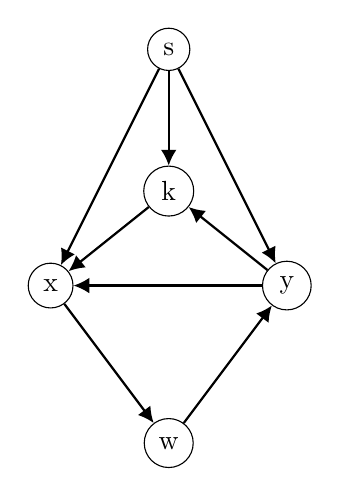
\begin{tikzpicture}
                \tikzset{vertex/.style = {shape=circle,draw,minimum size=1.5em}}
                \tikzset{edge/.style = {-{Latex[length=2mm,width=2mm]},thick}}
                
                \node[vertex] (s) at  (2.5,5) {s};
                \node[vertex] (x) at  (1,2) {x};
                \node[vertex] (y) at  (4,2) {y};
                \node[vertex] (w) at  (2.5,0) {w};
                \node[vertex] (k) at  (2.5,3.2) {k};
            
                \draw[edge] (s) -- (x);
                \draw[edge] (s) -- (y);
                \draw[edge] (x) -- (w);
                \draw[edge] (y) -- (k);
                \draw[edge] (y) -- (x);
                \draw[edge] (w) -- (y);
                \draw[edge] (k) -- (x);
                \draw[edge] (s) -- (k);
                
        \end{tikzpicture}
        \end{minipage}
        \textbf{$T_{tree}=(V, T) \Rightarrow$}
        \hfill
        \begin{minipage}{0.45\textwidth}
        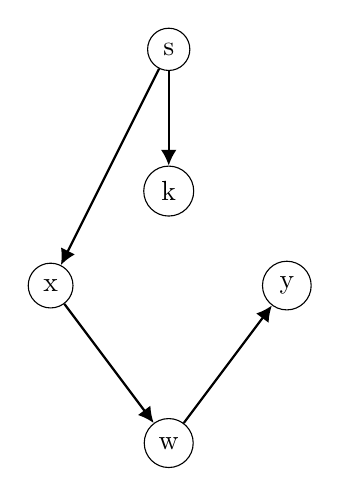
\begin{tikzpicture}
                
                \tikzset{vertex/.style = {shape=circle,draw,minimum size=1.5em}}
                \tikzset{edge/.style = {-{Latex[length=2mm,width=2mm]},thick}}
                
                \node[vertex] (s) at  (2.5,5) {s};
                \node[vertex] (x) at  (1,2) {x};
                \node[vertex] (y) at  (4,2) {y};
                \node[vertex] (w) at  (2.5,0) {w};
                \node[vertex] (k) at  (2.5,3.2) {k};
            
                \draw[edge] (s) -- (x);
                \draw[edge] (s) -- (k);
                \draw[edge] (x) -- (w);
                \draw[edge] (w) -- (y);
        
        \end{tikzpicture}
        \end{minipage}

  \color{black}

  \color{blue}
  \textbf{Justification:}\\
  \begin{enumerate}
    \item Both $(V, E)$ and $(V, T)$ are connected graphs.
    \item $|V|=5 \leq 5$.
    \item $T_{tree}$ forms a tree with root $s$.
    \item It is impossible to get $T_{tree}$ from graph $\mathcal{G}_3$ using \textbf{BFS} because at least there is no connection \textbf{s$\Rightarrow$y}. Since we start with \textbf{s}, each adjacency vertex must be visited.
    \item DFS cannot be applied. Let's try to represent T.\\ 
1) If we start with \textbf{$s \Rightarrow x \Rightarrow w \Rightarrow y \Rightarrow k$}, our algorithm will end with \textbf{k}, creating just a chain. We couldn't stop at \textbf{y} because we could go even deeper.\\
2) If we start with \textbf{$s\Rightarrow k\Rightarrow x\Rightarrow w\Rightarrow y$}, our algorithm will end with \textbf{y}, creating just a chain. We couldn't stop at \textbf{k} because we could go even deeper.
  \end{enumerate}
  \color{black}
  
\end{enumerate}

\begin{thebibliography}{BoasWrench}

\bibitem[CLRS]{Cormen2022}
Cormen, T.H., Leiserson, C.E., Rivest, R.L. and Stein, C., 2022. \emph{Introduction to algorithms, Fourth Edition}. MIT press.

\bibitem[GTG]{Goodrich2014}
M. T. Goodrich, R. Tamassia, and M. H. Goldwasser. \emph{Data Structures and Algorithms in Java.} WILEY 2014.

\end{thebibliography}

\end{document}